\documentclass[11pt]{article}
\usepackage[hmargin=1in,vmargin=1in]{geometry}
\usepackage{xcolor}
\usepackage{amsmath,amssymb,amsfonts,url,sectsty,framed,tcolorbox,framed,graphicx}
\newcommand{\pf}{{\bf Proof: }}
\newtheorem{theorem}{Theorem}
\newtheorem{lemma}{Lemma}
\newtheorem{proposition}{Proposition}
\newtheorem{definition}{Definition}
\newtheorem{remark}{Remark}
\newcommand{\qed}{\hfill \rule{2mm}{2mm}}

\begin{document}
\noindent
\rule{\textwidth}{1pt}
\begin{center}
{\bf [CS304] Introduction to Cryptography and Network Security}
\end{center}
Course Instructor: Dr. Dibyendu Roy \hfill Winter 2022-2023\\
Scribed by: Srushti Rathva (202051183) \hfill Lecture (Week 4)
\\
\rule{\textwidth}{1pt}

%week-4
\section*{Attack Models}
\subsection*{Ciphertext only Attack}
Attacker \textbf{knows only ciphertexts}. \\
\textbf{Goal} : Recover the plaintexts corresponding to the ciphertexts or recover the secret key.

\subsection*{Known plaintext Attack}
Attacker \textbf{knows some plaintexts} and corresponding \textbf{ciphertexts}. \\
\textbf{Goal} : Generate new plaintext, ciphertext pairs or recover the secret key.

\subsection*{Chosen plaintext Attack}
Attacker \textbf{chooses plaintexts} according to her/his choice and she/he will be given corresponding \textbf{ciphertexts}. \\
\textbf{Goal} : Generate new plaintext, ciphertext pairs or recover the secret key.

\subsection*{Known ciphertext Attack}
Attacker \textbf{chooses ciphertexts} according to her/his choice and she/he will be given corresponding \textbf{plaintexts}. \\
\textbf{Goal} : Generate new plaintext, ciphertext pairs or recover the secret key.

\section*{Breaking Secret Key}
\subsection*{Brute Force Approach}
One way we can break the secret key is that check for every secret key \\
This approach would require $2^{56}$ checks. 

\subsection*{Optimised Approach}
We know that, \\
DES(M,K) = C \\
DES($\bar{M}$,$\bar{K}$) = $\bar{C}$ \\ \\
Attacker chooses two plaintexts : \\
1.M and 2.$\bar{M}$ \\
$C_{1}$ = DES(M,K) \\
$C_{2}$ = DES($\bar{M}$,K) \\ \\
DES($\bar{\bar{M}}$,$\bar{K}$) = $\bar{C_{2}}$ \\
DES(M,$\bar{K}$) = $\bar{C_{2}}$ \\ \\
Attacker selects $K_{1} \in Keys$ \\
Attacker knows $\bar{K_{1}} \in Keys$ \\ \\
Perform DES(M,$K_{i}$) = $\bar{C}$ \\
if $\bar{C} \neq C{1}$ or $\bar{C} \neq \bar{C{2}}$ \\
Discard $K_{i}$ and $\bar{K_{i}}$ \\ \\
Hence, in every iteration attacker is checking two keys. \\
This approach would require $2^{55}$ checks.\\

\section*{Enhancing Security of DES}
DES is not secure due to multiple attacks. \\
We'll try to increase security by increasing length of secret key. \\

\subsection*{Double Encyption}
K = $K_{1} || K_{2}$ \\
len($K_{1}$) = len($K_{2}$) = 56 bits \\
len(K) = 112 bits \\ \\
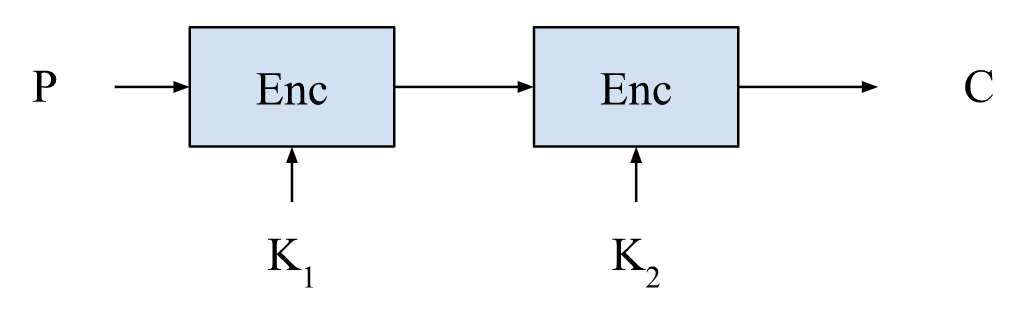
\includegraphics[width=300pt]{p1.png} \\ \\
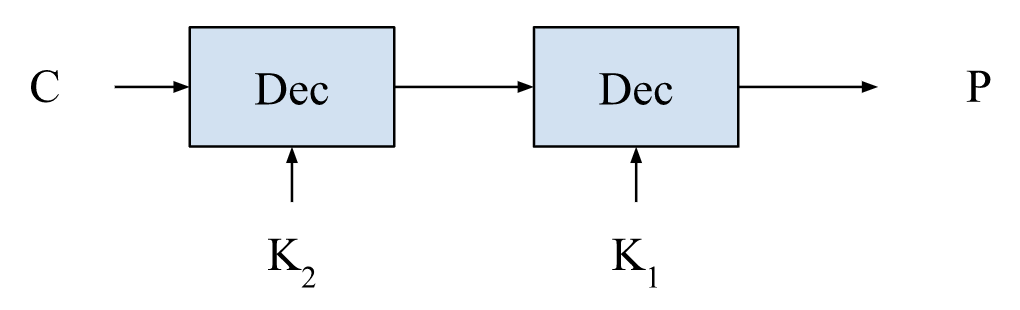
\includegraphics[width=300pt]{p2.png} \\ \\
Similarly other compositions are : EE,ED,DE,DD \\ \\
Attacker knows plaintext M and corresponding ciphertext C. \\
C = Enc(Enc(M,$K_{1}$),$K_{2}$) \\
Enc(M,S$K_{i}$) = $X_{i}$ \\
Dec(C,S$K_{j}$) = $Y_{j}$ \\
if $X_{i}$ = $Y_{j}$, then K = $SK_{i} || SK_{j}$ \\ \\
From here, we notice that double encryption does not enhance the security of DES. \\

\subsection*{Triple Encryption}
K = $K_{1} || K_{2}$ \\
len($K_{1}$) = len($K_{2}$) = 56 bits \\
len(K) = 112 bits \\ \\
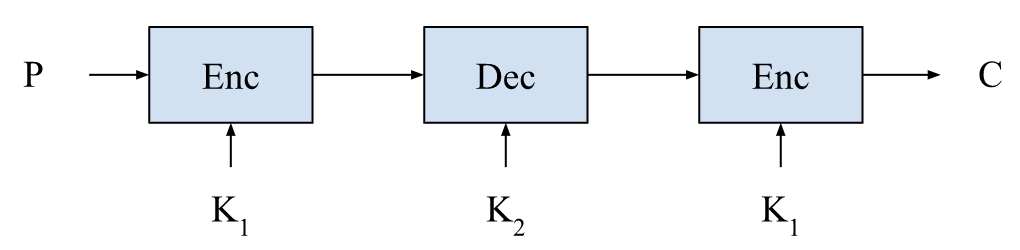
\includegraphics[width=350pt]{p3.png} \\ \\
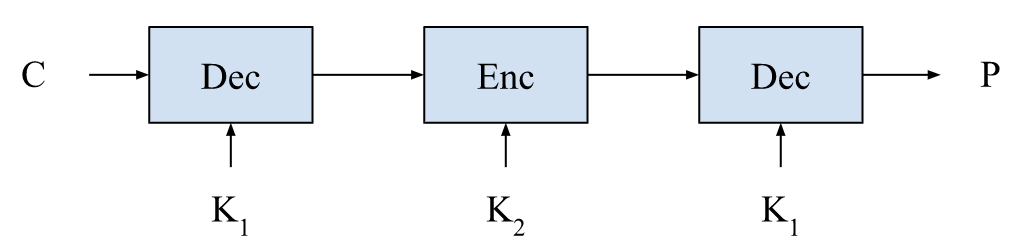
\includegraphics[width=350pt]{p4.png} \\ \\
Similarly other compositions are : EEE,EDE,DED and so on... \\ 
If DES is used with triple encryption, it is called Triple DES or 3-DES. 

\section*{Prerequisites}
\subsection*{Binary Operations}
It is a mapping from S$X$S to S. \\
$*$ : S$X$S $\rightarrow$ S

\subsection*{Groups}
It consists of a set G with defined binary operation * on G, satisfying following axioms : \\
 1. $*$ is associative on G. \\
 2. $\exists$ e$\in$G, which is an identity element. \\
 3. For each a$\in$G, $\exists$ $a^{-1}$ which is an inverse of a. \\ \\
 A group G is called obelion or commutative if, \\
 a*b = b*a $\forall$ a,b $\in$ G.
 
\end{document}
